%\vspace{-0.28cm}
\section{Fragment Transforms}
\label{sec:transforms}
%\vspace{-0.38cm}
The projection of objects onto images undergo an onslaught of visual transformations, as illumination, object pose, viewing distance or direction, \etc vary. In many cases contours extracted from images do not map to a complete object silhouette: gaps and clutter edges abound or internal contours due to 3D folds and self-occlusion, and contours due to partial occlusions. Our goal in this paper is to obtain parts whose shape and appearance is distinct and recognizable. Thus, gaps must be completed, spurious
contours removed, fragments across occlusions connected, \etc
This paper argues that there are significant advantages to casting these operations as transforms on the medial fragment as opposed to grouping contour fragments or regions. A sequence of medial transforms  then represents a perceptual grouping operation. We illustrate these below. 

\begin{figure*}[ht]
\centering
%\vspace{-0.75cm}
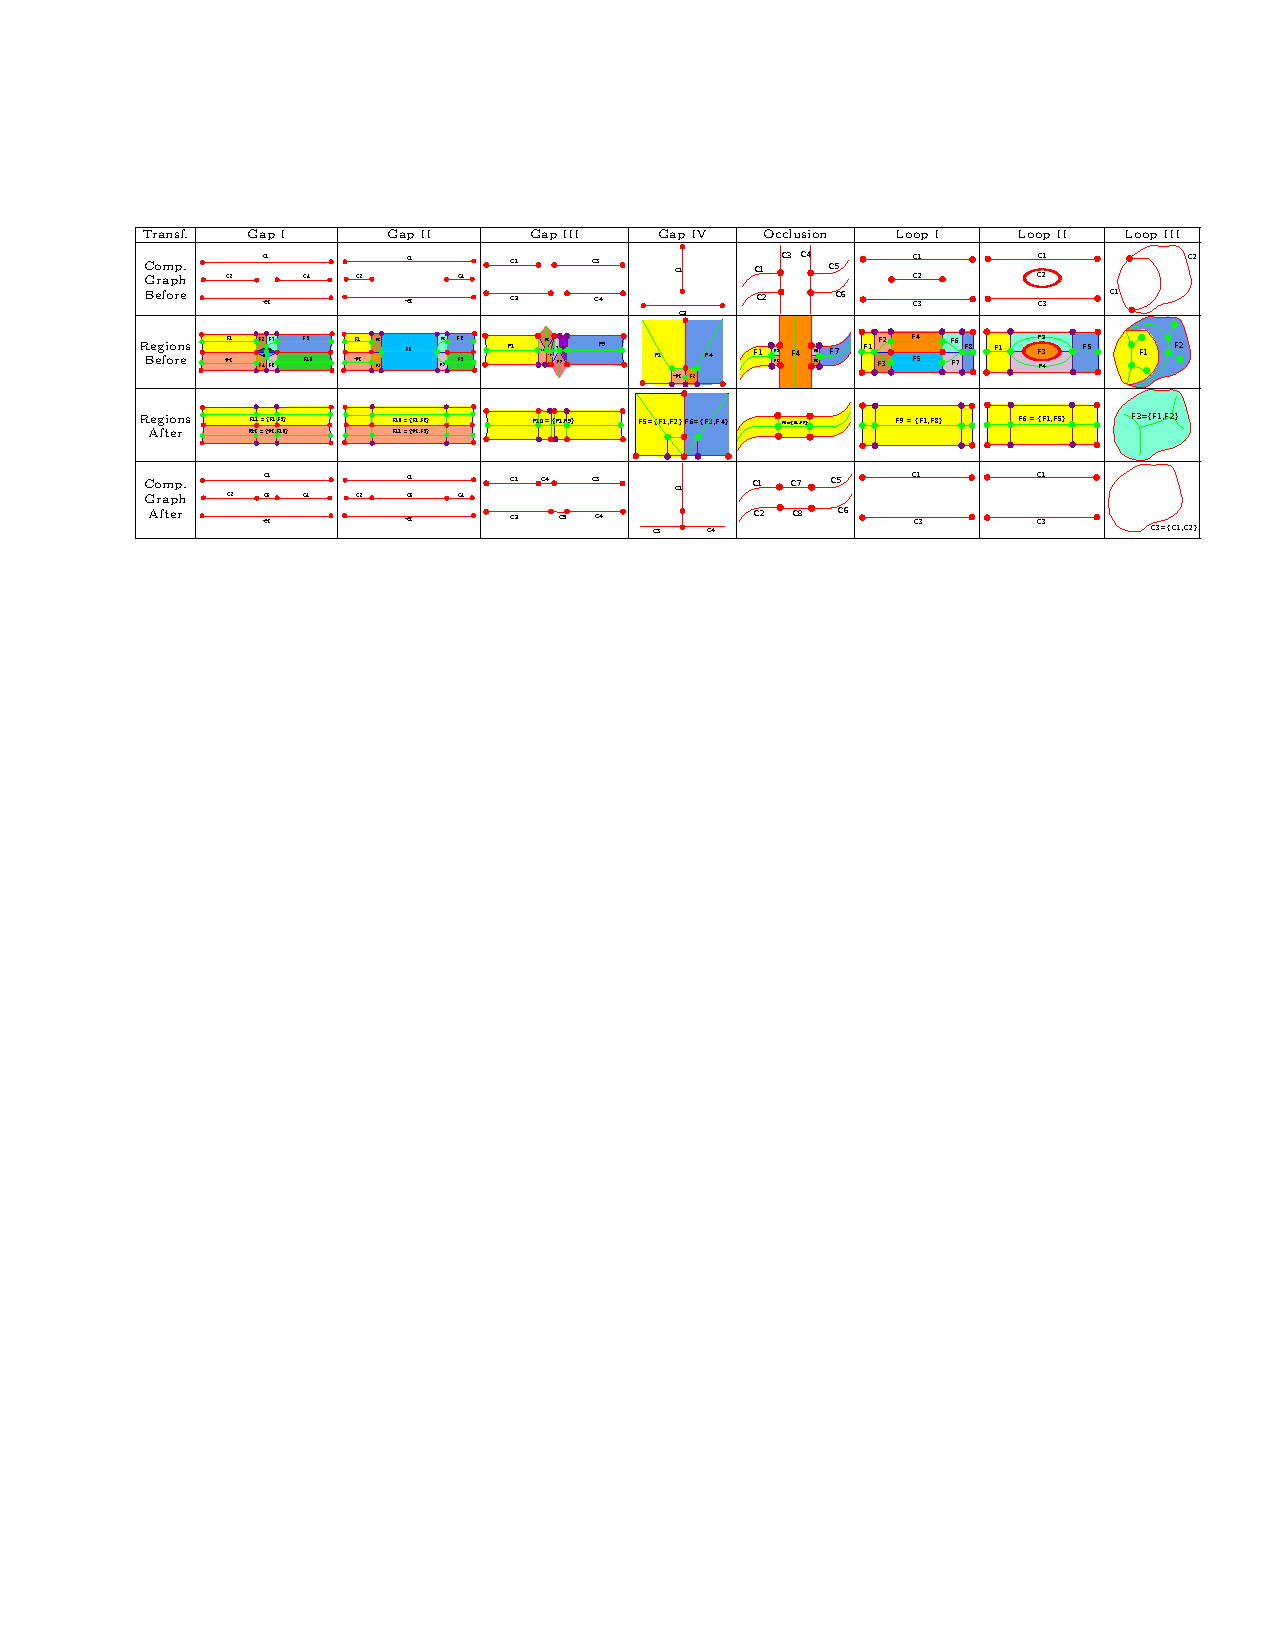
\includegraphics[width=1.0\linewidth]{figs/list-of-transforms.pdf}
%\vspace{-0.85cm}
  \caption{A partial list of transforms, arranged in columns. }
  \label{fig:transform:list}
  %\vspace{-0.75cm}
\end{figure*}

\textbf{Gaps} are those portions of veridical contour which did not make it through the contour
extraction process. As such, each gap leaves behind a pair of \textit{end-points}, or a single end-point if the gap is at a junction. The remedy is simple:\ complete the contour
between two end-points by interpolation. However, which of the many pairing of end points  should  be completed? To aid in the selection process, we augment the well-known Gestalt cue of {\em contour continuity} with two other proposed cues: {\em figural continuity} and {\em appearance continuity}.
The medial fragment representation makes this possible, since the template in the first column of Figure~\ref{fig:transform:list} will not form if
there are intervening contours. Specifically {\em (i)} contour continuity
is formulated in by Euler Spiral energy~\cite{Kimia:Euler:Spiral:IJCV03}
with  variables $\{\gamma, \kappa_0,l\}$, where $\gamma$, $\kappa_0$, and $l$ represent derivative of curvature, initial curvature, and arc-length
of the completion curve. The parameters of the energy function are learned
under supervised learning using a generalization of the Geisler model~\cite{Geisler:Vision:Journal};
{\em (ii)} figural continuity is formulated by comparing the radius of the medial
axis for fragments F1 and  F9, and F2 and F10, respectively; {\em (iii)} Appearance
continuity ensures that the appearance of fragments F1 and  F9, and F2 and F10, respectively is contiguous; we have not implemented the latter
cue at the moment. The first two cues associate a likelihood with each GAP I Transform. For a recent perceptual study of gap completion see~\cite{Narayanan:Kimia:POCV12}.



The remaining two types of gaps are essentially the same modulo differences in gap width
and end-point arrangement.  The fourth type of gap arises from a junction, but it is essentially
handled in the same way. There is also an dis-occlusion transform which
is essentially a gap in the figure.  


\begin{figure}[!h]
%\vspace{-0.3cm}
\hspace{-0.051cm}\footnotesize{\textit{a}} 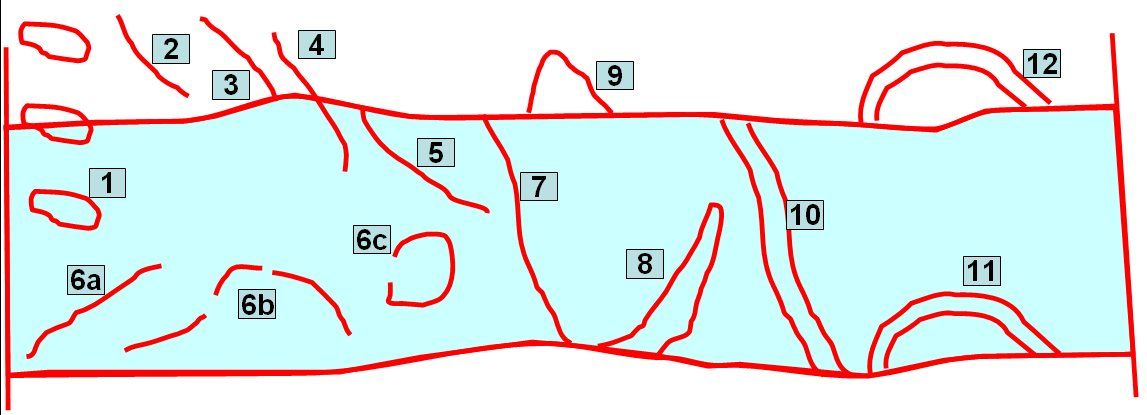
\includegraphics[height=0.06\linewidth]{figs/all-loop-cases.jpg}
\footnotesize{\textit{b}}\hspace{-0.0051cm}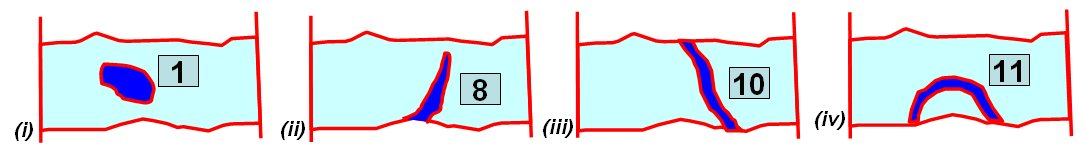
\includegraphics[height=0.06\linewidth]{figs/refined-all-loop-cases-1.jpg}
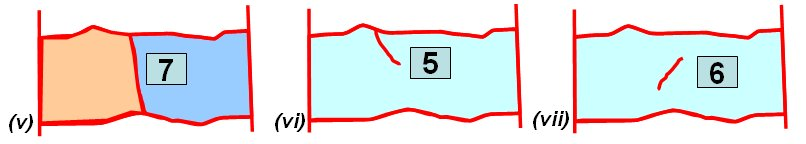
\includegraphics[height=0.06\linewidth]{figs/refined-all-loop-cases-2.jpg}
\centerline{
%\includegraphics[width=0.10\linewidth]{figs/fragment-no-contamination.jpg}
 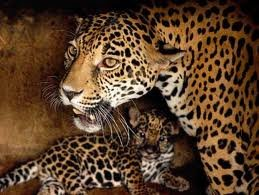
\includegraphics[height=0.110\linewidth]{figs/leopard.jpg}
 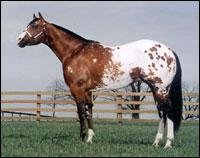
\includegraphics[height=0.110\linewidth]{figs/horse61.jpg} 
 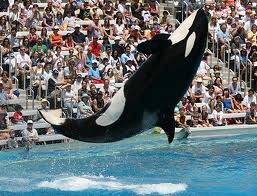
\includegraphics[height=0.110\linewidth]{figs/shamu-1.jpg}
 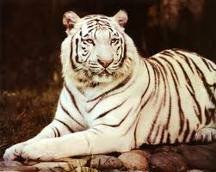
\includegraphics[height=0.110\linewidth]{figs/tiger-1.jpg}  
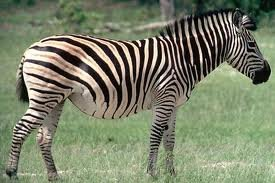
\includegraphics[height=0.110\linewidth]{figs/zebra-1.jpg}
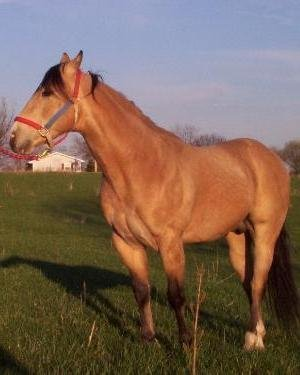
\includegraphics[height=0.110\linewidth]{figs/horse6.jpg}  
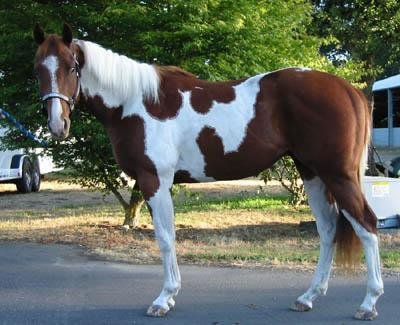
\includegraphics[height=0.110\linewidth]{figs/horse49.jpg}  
}
%\vspace{-0.6cm}
\caption{\FigureFont (a)We use a sketch of a normative object part, the horizontal cyan
strip, to systematically derive all possible ways a spurious contour can
 interfere with its formation, leading to  seven
principal cases, as in(b). These can be easily recognized in natural images (c), \eg, leopard spots, markings off a whale, tiger stripes,
\etc Our set of 
loop transforms correspond to the removal of their effect so that object part hypotheses can form.}
   \label{fig:loop:transforms}
   %\vspace{-0.75cm}
\end{figure}

\textbf{Spurious Contours} are those contour fragments that do not belong to the object part boundaries, although they often explain the 3D local form, object texture, reflectance, \etc
They are only spurious in the sense that they interfere with the formation of an object part. A syntactic account of how spurious contours can interfere with the formation of object part boundaries in seven canonical cases is shown in Figure~\ref{fig:loop:transforms}a-b. On all cases the shock graph has a loop corresponding to the interfering element which can be removed by the application of one of the three loop transforms shown in Figure~\ref{fig:transform:list}.  

The remaining transforms are similarly intuitive embodiments of known Gestalt grouping
operations and will not be further explained here. It is possible that additional transforms arise with additional experience  with this approach, but the ones listed are the major ones. This language of transforms is powerful enough to be able to organize tiger parts from the very challenging tiger image, Figure~\ref{fig:tiger:sequence}. 
  


% \begin{figure}[!h]
% %\centerline{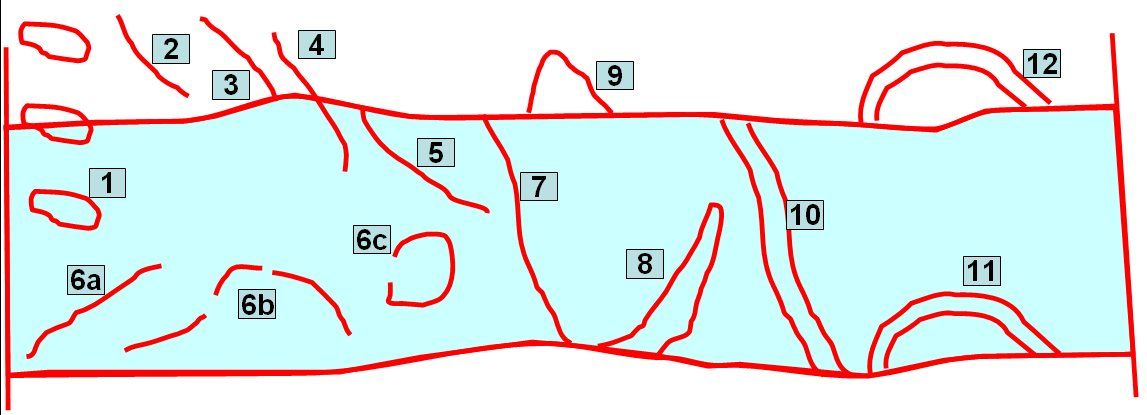
\includegraphics[width=0.5\linewidth]{figs/all-loop-cases.jpg}}
% \centerline{
%  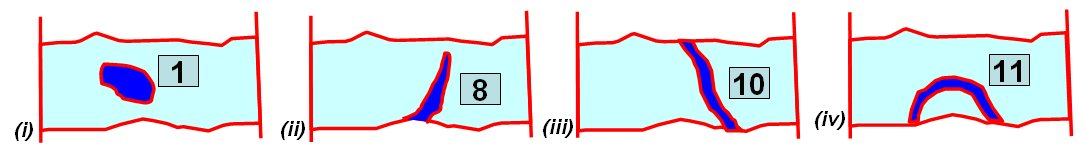
\includegraphics[height=0.0846\linewidth]{figs/refined-all-loop-cases-1.jpg}
%     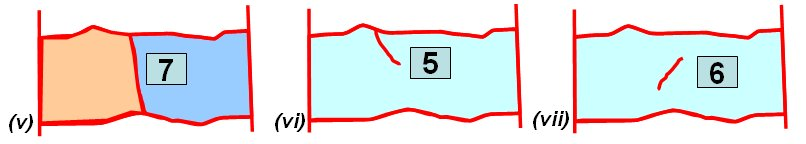
\includegraphics[height=0.0846\linewidth]{figs/refined-all-loop-cases-2.jpg}}
%  \centerline{
% \footnotesize{\textit{i)}}
%  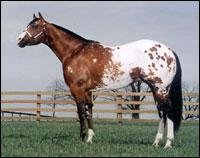
\includegraphics[height=0.1\linewidth]{figs/horse61.jpg} 
%  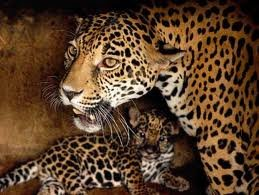
\includegraphics[height=0.1\linewidth]{figs/leopard.jpg}
% \footnotesize{\textit{ii)}}
%  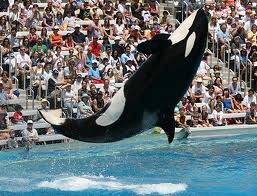
\includegraphics[height=0.1\linewidth]{figs/shamu-1.jpg}
%  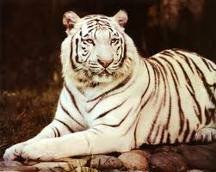
\includegraphics[height=0.1\linewidth]{figs/tiger-1.jpg}
%  \footnotesize{\textit{iii)}}      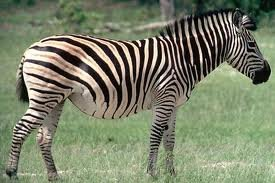
\includegraphics[height=0.1\linewidth]{figs/zebra-1.jpg}
%  % \footnotesize{\textit{(iv)}} \includegraphics[height=0.1\linewidth]{figs/replace-me.jpg}
%  \footnotesize{\textit{v)}}  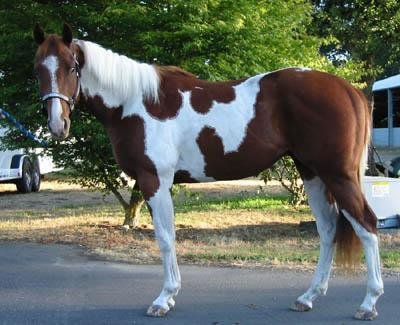
\includegraphics[height=0.1\linewidth]{figs/horse49.jpg}
%  \footnotesize{\textit{vi)}}  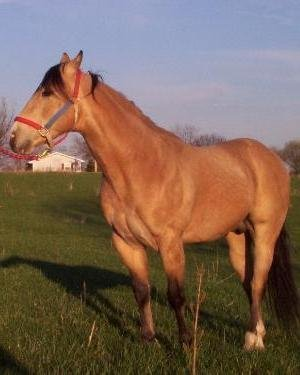
\includegraphics[height=0.1\linewidth]{figs/horse6.jpg}}
% \caption{\FigureFont Examples of a classification of contour fragments interacting with an existing fragment. }
%    \label{fig:all-loop-cases-examples}
% \end{figure}
 



A critical issue in exploring alternative perceptual organization is to associate a likelihood to each transform sequence so that only plausible cases can be explored. Assuming independence among transforms, the likelihood a transform sequence forms a valid fragment is 
%\vspace{-0.3cm}
\begin{equation}
%\vspace{-0.3cm}
p(T_1,T_2,...,T_N)=\prod_i^Np(T_i)
\label{eq:path_like}
\end{equation}
where $p(T_i)$ represents the likelihood of a transform and $p(T_1,T_2,...,T_N)$ is a transform sequence. See supplementary section for further technical details. % \begin{figure}[!h]
%   \centering
% %   \includegraphics[width=.13\textwidth]{figs/tiger-figs/transform/start_tiger.jpg}
% %   \includegraphics[width=.13\textwidth]{figs/tiger-figs/transform/tiger1.pdf}
% %   \includegraphics[width=.13\textwidth]{figs/tiger-figs/transform/tiger2.pdf}
% %   \includegraphics[width=.13\textwidth]{figs/tiger-figs/transform/tiger3.pdf}
% %   \includegraphics[width=.13\textwidth]{figs/tiger-figs/transform/tiger4.pdf}
% %   \includegraphics[width=.13\textwidth]{figs/tiger-figs/transform/tiger5.pdf}
% %   \includegraphics[width=.13\textwidth]{figs/tiger-figs/transform/end_tiger.jpg}
% %\includegraphics[width=.51\textwidth]{figs/tiger-transform-areas.jpg}
%   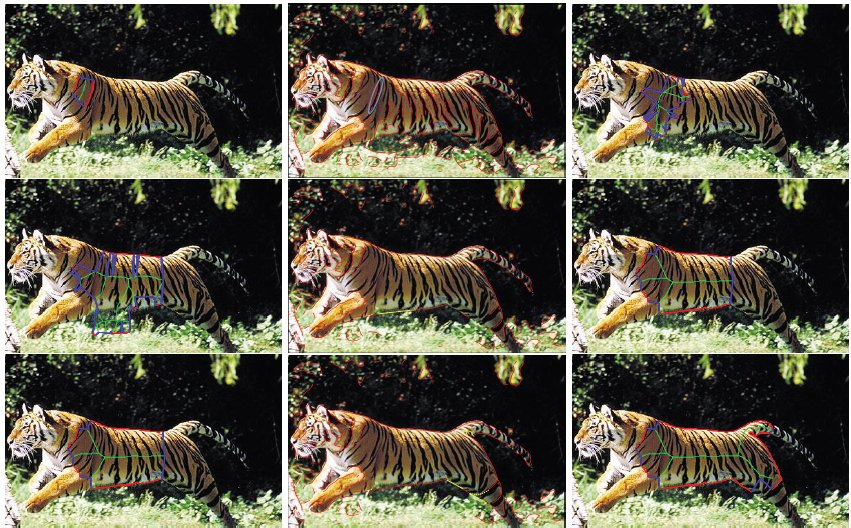
\includegraphics[width=.51\textwidth]{figs/tiger-transform-examples.jpg}
%   \caption{\small Three examples of the Transforms applied.}
%   \label{figure:tiger_transforms}
%   %\vspace{-0.5cm}
% \end{figure}

% \begin{figure*}[t]
%   \centering
%    \includegraphics[width=.8\textwidth]{figs/tiger_seq.pdf}
%   \caption{\small A sequence of transforms on the tiger image.}
%   \label{fig:tiger:sequence}
%   %\vspace{-0.15cm}
% \end{figure*}
% 
% \begin{figure}[t]
%   \centering
%   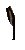
\includegraphics[width=.025\textwidth]{figs/tiger1_f.jpg}
%   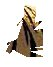
\includegraphics[width=.05\textwidth]{figs/tiger2_f.jpg}
%   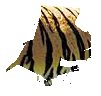
\includegraphics[width=.075\textwidth]{figs/tiger3_f.jpg}
%   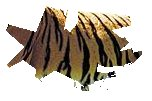
\includegraphics[width=.1\textwidth]{figs/tiger4_f.jpg}
%   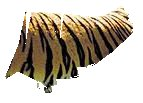
\includegraphics[width=.1\textwidth]{figs/tiger5_f.jpg}
%   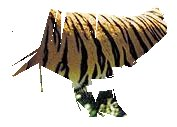
\includegraphics[width=.1\textwidth]{figs/tiger6_f.jpg}
%   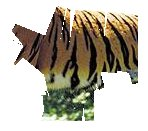
\includegraphics[width=.1\textwidth]{figs/tiger7_f.png}
%   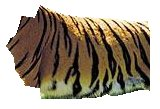
\includegraphics[width=.1\textwidth]{figs/tiger8_f.png}
%   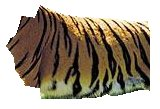
\includegraphics[width=.1\textwidth]{figs/tiger8_f.png}
%   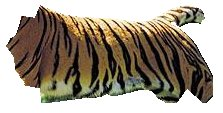
\includegraphics[width=.1\textwidth]{figs/tiger10_f.png}
% 
%   \caption{\small Sequence of fragment formation on the tiger image. }
%   \label{figure:tiger_frag_type}
%\end{figure}
